\subsection{PCB}
\label{subsec:PCB}
Ein PCB (Printed Circuit Board, dt. Leiterplatte) beherbergt die verwendeten Bauteile und verbindet diese elektronisch miteinander. Die verwendeten Bauteile werden auf das PCB gelötet, wobei es SMD (Surface Mount Device) und THT (Trough Hole Technology) zu unterscheiden gilt. Wie der Name schon sagt, werden THT-Bauteile durch das PCB gesteckt und SMD-Bauteile lediglich auf die Oberfläche gelegt, wobei beide vorgesehene Lötstellen haben auf diese sie gelötet werden um elektrischen Kontakt über Leiterbahnen zu erstellen.
Das PCB und das dazugehörige Schema werden in einem EDA-Programm (Electronic Design Automation) erstellt. Für die Wetterstation wurde das Programm EAGLE (Einfach Anzuwendender Grafischer Layout-Editor) der Firma Autodesk verwendet, wegen der im Namen schon angedeuteten einfachen Anwendung. Für die Wetterstation wurde ein 4-Lagen-PCB ausgewählt, da dies im Vergleich zu einem 2-Lagen-PCB zu einem einfacheren Entwurf verhilft, hauptsächlich in Bezug zu Stromrückflüssen und EMV. Das Schema und das dazugehörige PCB-Layout sind im Anhang zu finden (Schema in Kapitel \ref{Anhang:Schema}, PCB-Layout in Kapitel \ref{Anhang:PCB}). Dem Anhang ist zu entnehmen, dass der erste und der vierte Layer für Signale bestimmt sind, der dritte Layer für die Versorgung (+3.3V) und der zweite Layer für das Ground (0V). In den nachfolgenden Abschnitten wird auf das Bestücken der Leiterplatte eingegangen und auf Mängel der ersten Version hingewiesen, sowie die Art und Weise wie diese Mängel behoben wurden.
\subsubsection{Das Bestücken der Leiterplatte}
{\begin{minipage}[b][6cm][t]{0.4\textwidth}
THT Bauteile werden durch das PCB durchgesteckt und von unten her angelötet. Nach dem anlöten werden die Beine, welche standardmässig relativ lang sind, möglichst nahe am PCB mit einem kleinen Seitenschneider gekürzt. In Abbildung \ref{fig:THT_Loeten} das Löten eines THT-Bauteils illustriert.
\end{minipage}}
{\begin{minipage}[b][6cm][t]{0.59\textwidth}
\centering
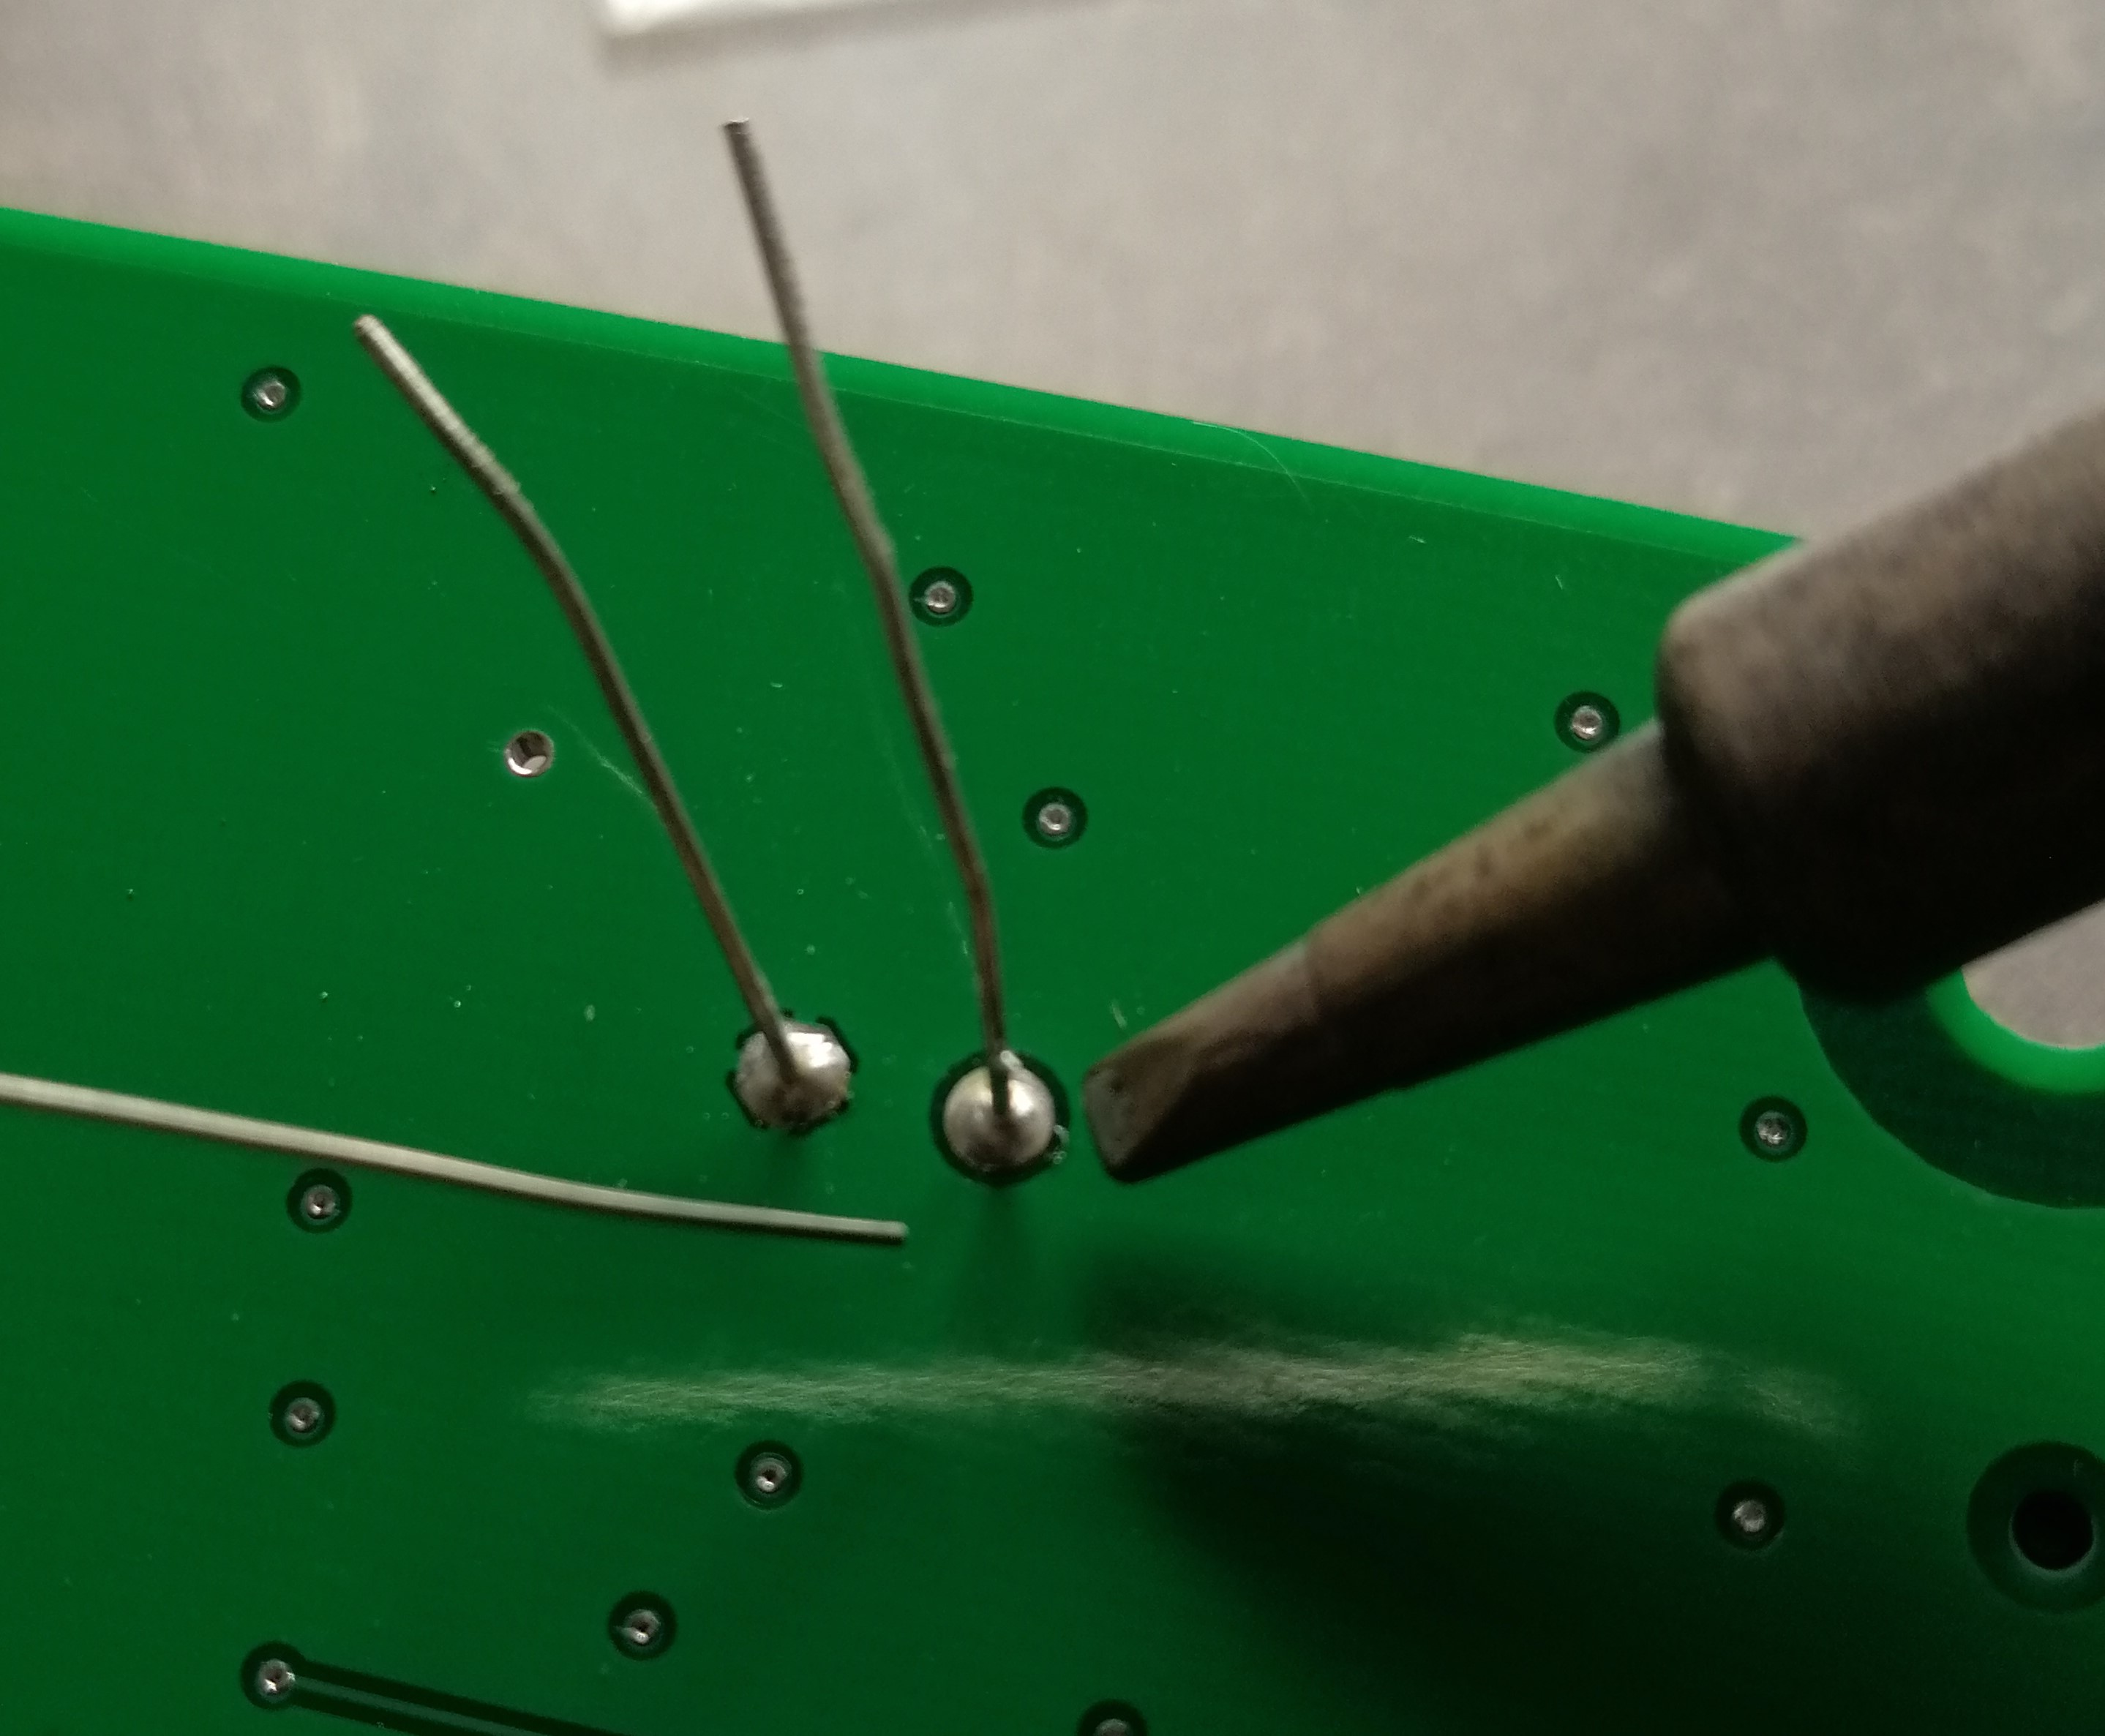
\includegraphics[width=0.7\linewidth]{graphics/HW_Val/THT_Loeten.jpg}
\captionof{figure}{Das Löten eines THT-Bauteils.}
\label{fig:THT_Loeten}
\end{minipage}}

{\begin{minipage}[b][8cm][t]{0.5\textwidth}
SMD Bauteile werden auf die Oberfläche des PCBs gelegt und dort angelötet. Dabei wird zuerst auf dem ersten Lötauge etwas Lötzinn aufgetragen. Mit einer Pinzette wird nun das SMD Bauteil korrekt platziert, während mit dem Lötstab der vorher aufgetragene Lötzinn flüssig gehalten wird. Ist das Bauteil korrekt platziert, wird es mit der Pinzette angedrückt, so dass es sich nicht verschiebt wenn der Lötstab entfernt wird und dieser dann entfernt, so dass der Lötzinn sich erhärtet und das Bauteil festhält. Nun kann von der anderen Seite her mit dem Lötstab das Lötauge erhitzt und mit Lötzinn das Bauteil angelötet werden. Dieser Vorgang wird in Abbildung \ref{fig:SMD_Loeten} illustriert.
\end{minipage}}
{\begin{minipage}[b][8cm][t]{0.49\textwidth}
\centering
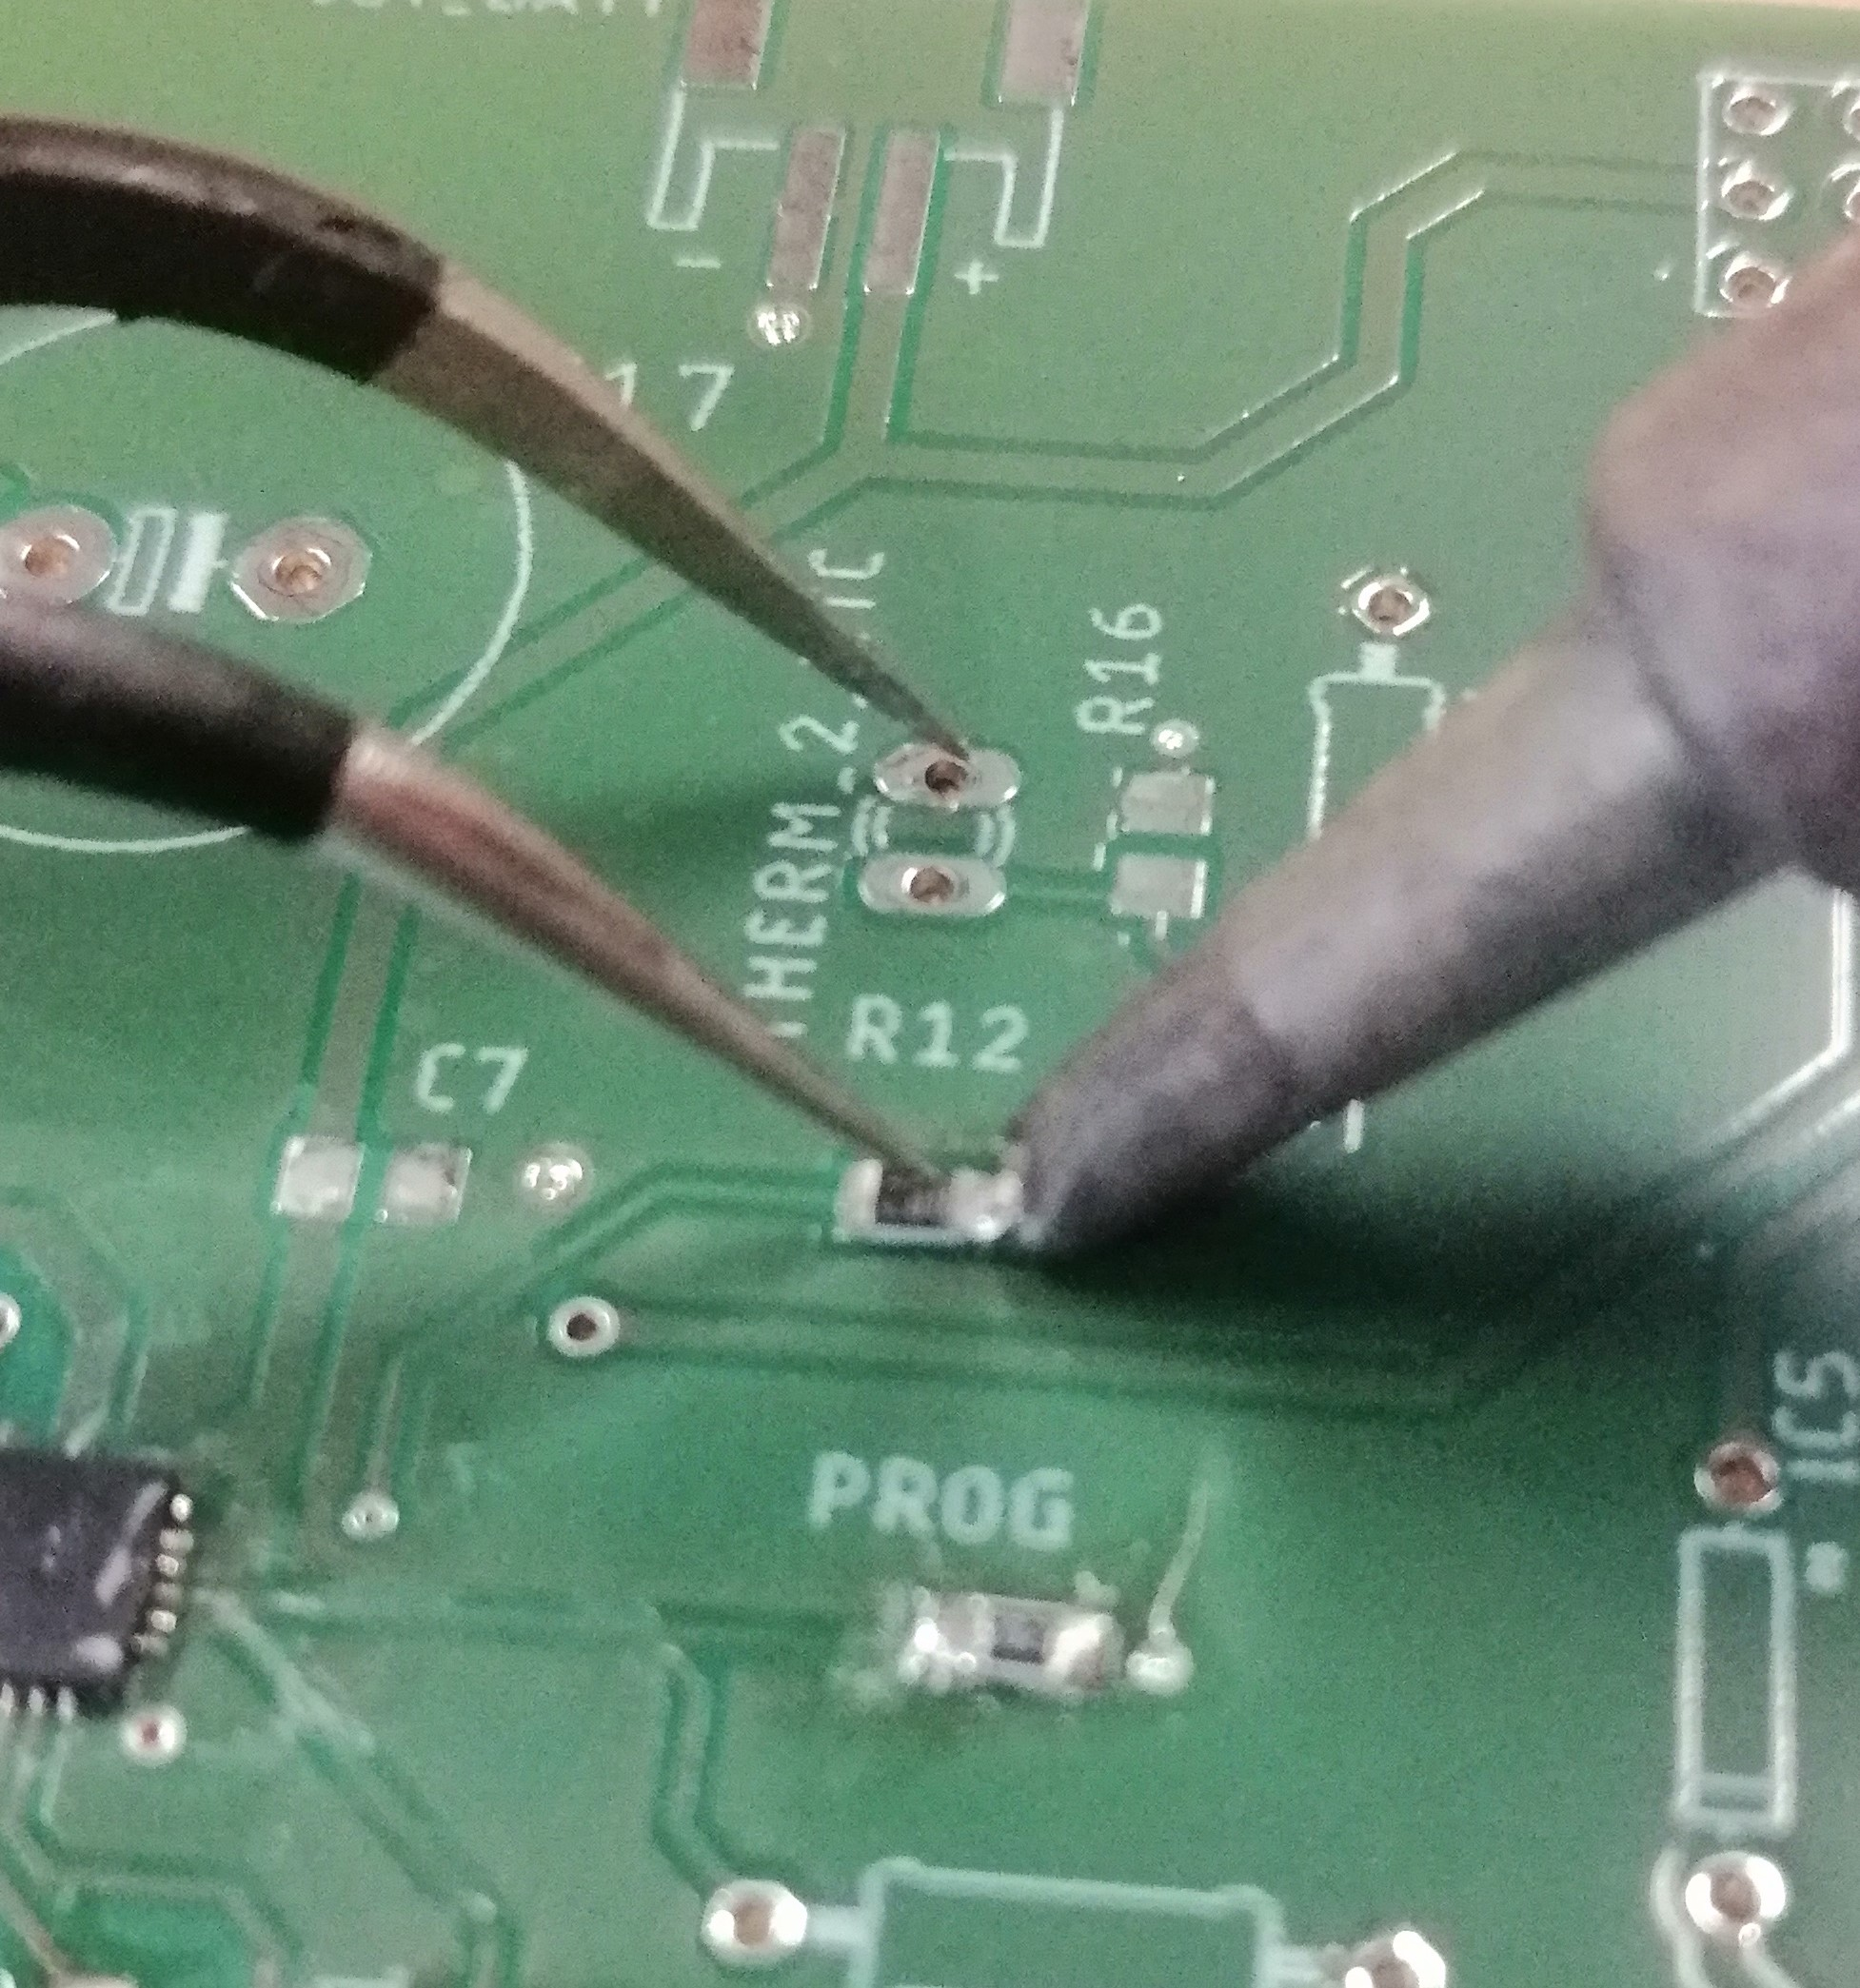
\includegraphics[width=0.8\linewidth]{graphics/HW_Val/SMD_Loeten.jpg}
\captionof{figure}{Das Löten eines SMD-Bauteils.}
\label{fig:SMD_Loeten}
\end{minipage}}


Die MCU hat ein TQFP gehäuse mit insgesamt 100 Pins (25 je Seite). Diese Pins sind äusserst nahe beieinander und sehr dünn, weshalb ein normales anlöten wie bei oben genannten SMD Bauteilen nicht gut funktioniert. Hier wird das oft \textit{Ziehlöten} genannte Verfahren angewendet. Dabei wird die MCU erst äusserst sorgfältig korrekt platziert. Mit einer Pinzette wird die MCU an Ort und Stelle gehalten. Die Pins auf einer Seite werden nun grosszügig mit Flussmittel eingestrichen. Direkt nach dem Einstreichen muss der Lötstab mit dem breiten Lötaufsatz und ganz wenig Lötzinn über die Pins fahren, um den Lötzinn auf die Pins zu verteilen. Nun kann wieder mit dem Flussmittel gearbeitet werden, wobei der Lötstab frontal von den Enden der Pins (MCU-seitig) nach aussen gzogen wird. Lötzinn muss im zweiten Schritt meistens keiner mehr verwendet werden und wenn doch, dann nur äusserst wenig. Die Kunst besteht darin, nicht zu viel Lötzinn zu verwenden, da sonst Lötbrücken entstehen können, welche nicht ganz einfach zu entfernen sind. Dieses Verfahren wird in den Abbildungen \ref{fig:MCU_Prep} und \ref{fig:MCU_Loeten} dargestellt.\\

{\begin{minipage}[b][8cm][t]{0.49\textwidth}
\centering
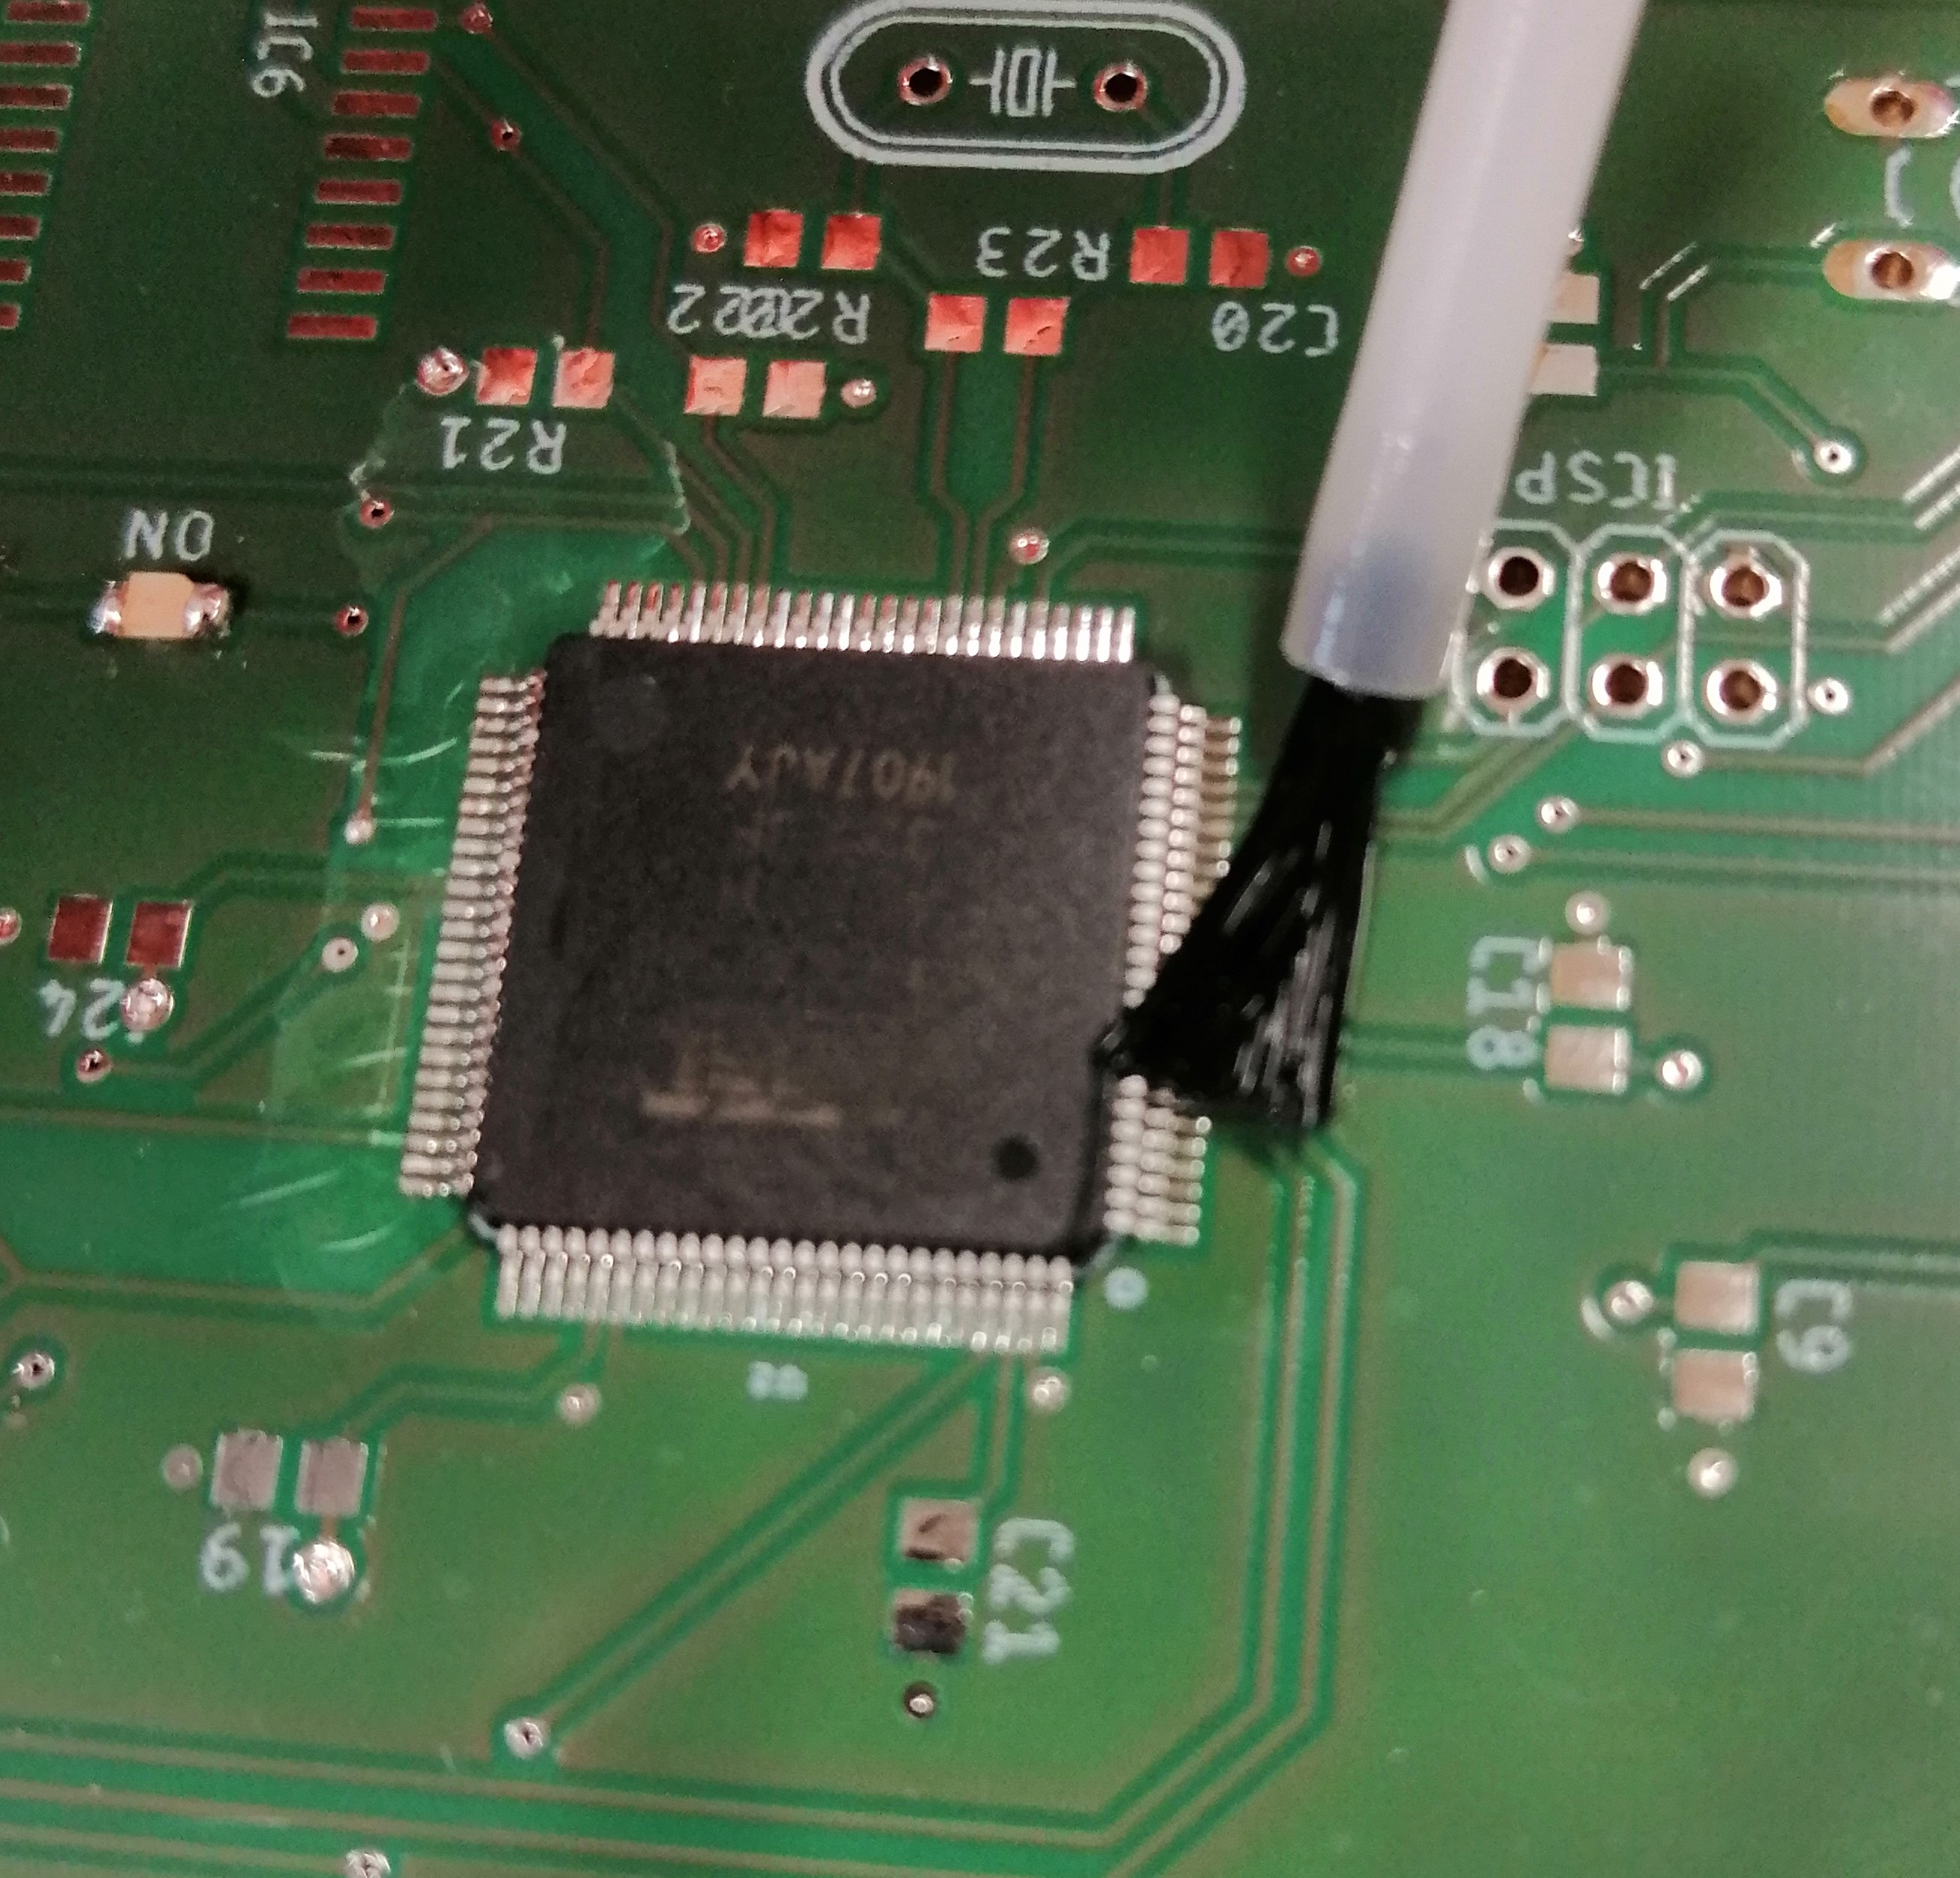
\includegraphics[width=0.9\linewidth]{graphics/HW_Val/MCU_Prep.jpg}
\captionof{figure}{Verteilen des Flussmittels an die Pins der MCU.}
\label{fig:MCU_Prep}
\end{minipage}}
{\begin{minipage}[b][8cm][t]{0.49\textwidth}
\centering
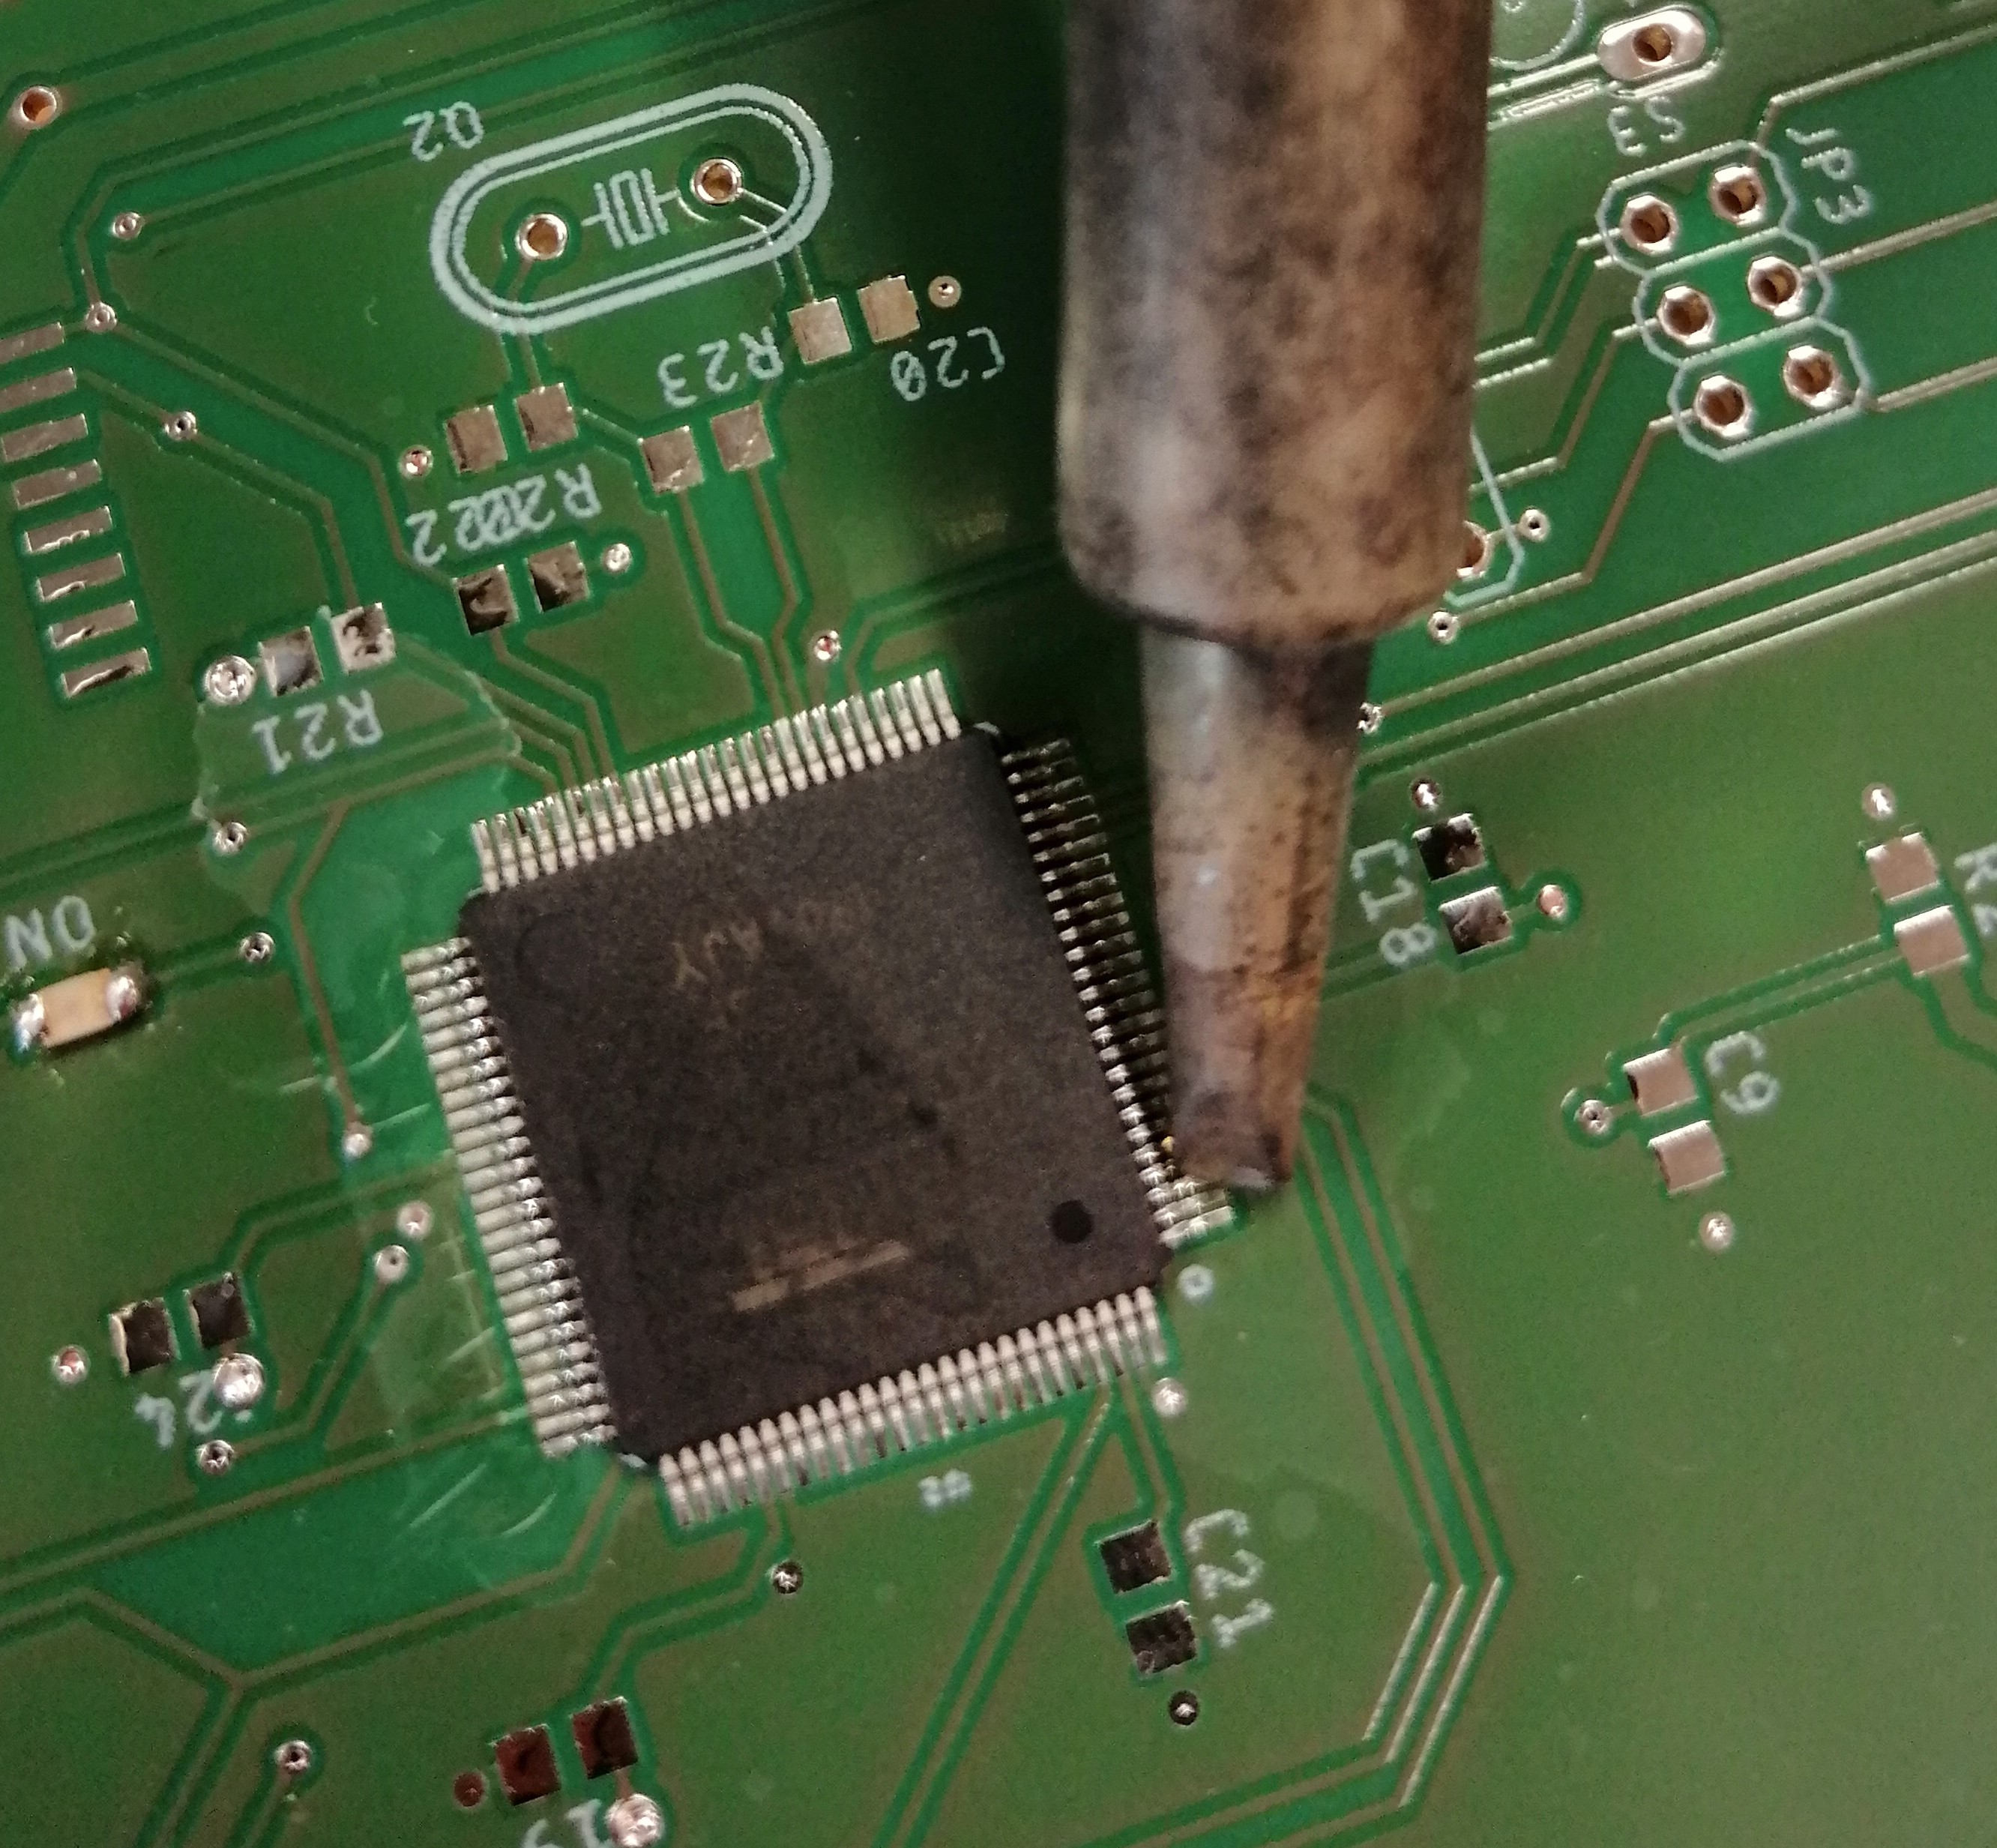
\includegraphics[width=0.9\linewidth]{graphics/HW_Val/MCU_Loeten.jpg}
\captionof{figure}{Löten der MCU via Ziehlötverfahren.}
\label{fig:MCU_Loeten}
\end{minipage}}
\newpage
Das Vorbereiten der Lötstellen der MCU mit der Zugabe des Flussmittels wird in Abbildung \ref{fig:MCU_Prep} dargestellt. Wichtig ist, dass dies unmittelbar vor dem Löten gemacht wird, da sich das Flussmittel an der Luft verflüchtigt. In Abbildung \ref{fig:MCU_Loeten} wird ersichtlich, dass der Lötkolben mit dem breiten Lötaufsatz über die Pins der MCU fährt. Dabei wird nur sehr wenig Lötzinn verwendet, um keine Brücken zwischen zwei Pins zu erstellen.

\subsubsection{Mängel der Erstversion und dessen Verbesserungen}
Die Mängel der Erstversion werden hier aufgelistet und deren Verbesserung für die Zweitversion direkt erläutert.
\begin{enumerate}
\item Beim ersten Testen des Boards wurde erkannt, dass Probleme mit dem Versorgungslayer bestehen, da fast alle Bauteile, welche mit diesem über ein Via (ein Verbinder zwischen Layer) verbunden sein sollten, nicht mit Strom versorgt wurden. Dieses Manko wurde provisorisch mit einer Leiterplatte und Drähten gelöst, so dass weitere Tests gemacht werden konnten.\\
Für die Zweitversion wurde die Füllung des Versorgungslayers mit direkten Leiterbahnen zu den entsprechenden Pins ersetzt.
\item In einem weiteren Schritt wurde erkannt, dass die ChargePump nicht die gewünschte Spannung ausgibt wie auf einem Steckbrett zuvor getestet, wobei sich dieser Mangel erst bei geringerem Akkustand bemerkbar macht, weshalb weitere Tests gemacht werden konnten.\\
Um dieses Problem zu beheben, sollen andere Dioden verwendbar sein, Aus diesem Grund werden für den zweiten Print THT-Bauteile verwendet, da diese einfacher auszulöten und zu ersetzen sind.
\item Gemäss den Tests sperren die Schutzdioden in der Nähe des DCIN Jacks nicht wie gewünscht in Sperrrichtung.\\
Auch hier werden für den zweiten Print THT-Bauteile verwendet, um ein austauschen der Dioden vornehmen zu können.
\item Pins für die serielle Schnittstelle (TXD und RXD) wurden vertauscht, weshalb keine Kommunikation über PuTTY erfolgen konnte.\\
Dieses Problem wurde im Redesign behoben, indem die Anschlüsse vertauscht wurden.
\item Beim SIM808 muss der Pin PWRKEY auf Ground sein um diesen starten zu können. Dieser Pin war jedoch nicht auf Ground gezogen sondern floating.\\
Der entsprechende Pin wurde im Redesign mit Ground verbunden.
\item Desweiteren konnte beim SIM808 die 1.8V Ausgangsspannung für die SIM-Karte nicht gemessen werden. Es wurde vermutet, dass es wegen des TVS-Arrays nicht möglich war. Für das TVS-Array wurde ein zu kleiner Footprint verwendet, weshalb die Lötaugen nicht zur Grösse des Gehäuses passte, was schliesslich zu defekten auf dem PCB führte.\\
Der Footprint wurde von Hand angepasst, so dass das Bauteil nun richtig angelötet werden kann. Ausserdem wurde eine Bestückungsvariante implementiert, mit der der SIM808 mit Breakout Board direkt angeschlossen werden kann über Pinheader.
\item Die Signale des Anemometers und des Ombrometers waren verrauscht, was auf einen ineffektiven Tiefpass hindeutet. Die Abstände zwischen Widerstand und Kondensator waren wirklich etwas weit entfernt.\\
Die Abstände wurden im Redesign massiv verringert.
\item Der verwendete Kippschalter trennt die Wetterstation von der Versorgung, jedoch ist der SIM808 direkt vom Akku gespiesen und läuft deshalb weiter.\\
Durch das Ersetzen des Kippschalters mit einem anderen, welcher 2 Stromkreise gleichzeitig schaltet, konnte dieses Problem im Redesign behoben werden.
\end{enumerate}
Die Mängel wurden gemäss den Erläuterungen behoben und ein zweites PCB bestellt. Das eingetroffene PCB wies weiterhin Problem 1 auf, was erst zu Ratlosigkeit führte. Schnell konnte jedoch herausgefunden werden, dass der Hersteller des PCBs (JLCPCB) keine Blind Vias unterstützt, welche jedoch für die Verbindung zwischen Bauteil und Versorgungslayer im Design verwendet wurden. Es musste deshalb ein drittes PCB bei einem Hersteller bestellt werden, welches Blind Vias unterstützt. Auf der Webseite www.multi-circuit-boards.eu konnten Blind Vias als Option angekreuzt werden, weshalb bei diesem Hersteller das dritte PCB bestellt wurde. Bestellen musste dies jedoch die FHNW, da dieser Anbieter nur an Institutionen und Unternehmen liefert und die Projektteilnehmer die kosten eines PCBs von rund 280.- nicht auf sich nehmen konnten. \\[0.5cm]
Das erfolgreich erhaltene dritte PCB wurde wie erläutert bestückt und getestet gemäss den dokumentierten Tests in Kapitel \ref{subsubsec:HW_Val}. Die Wetterstation funktioniert soweit und benötigt lediglich ein Gehäuse, um präsentabel zu sein und um ein Betrieb im Freien zu ermöglichen. Auf diese Thematik wird im nächsten Kapitel eingegangen.
